% Homework #5
% COSC552 HCI
%
% Byron Heads
% E00062946

\documentclass[12pt]{report}

\usepackage{graphics}
\usepackage{hyperref}

\title{Homework Set 5 \\
    COSC552 HCI}
\author{ Byron Heads \\
    E00062946 }
\date{\today}

\begin{document}
\maketitle

\chapter*{A}

The search engine design I use is based on a mix between free-form, and 
a defined search.  The user is able to search for a keyword or phrase
on the entire database, or they can limit their results by searching only
in a category.  This allows a user to do complex searches without learning
advanced search syntax.

\begin{figure}[h!]
\center{\resizebox{280pt}{!}{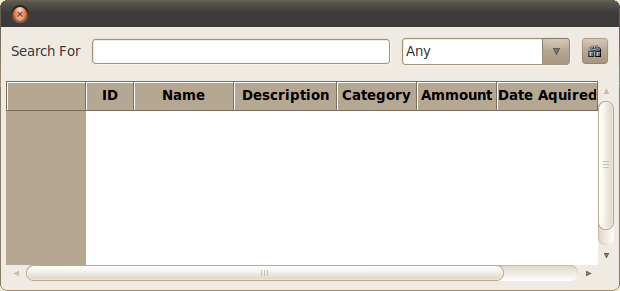
\includegraphics{ss1.png}}}
\caption{A Prototype search dialogbox.}
\end{figure}

The user can enter the keyword they wish to search for in the first textbox
and then select which category they would like to search in.  The default
category is Any, which searches all categories.

\begin{figure}[h!]
\center{\resizebox{280pt}{!}{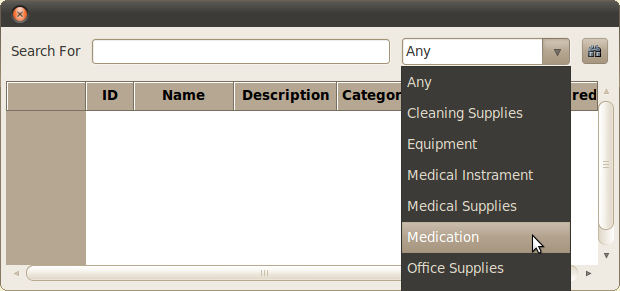
\includegraphics{ss2.png}}}
\caption{The category menu shows the top categories in the database.  The
number shown is limited by a setting in the configuration menu.  Top 
categories are based off number of items in that category and how often
items in that category are searched for.}
\end{figure}

\chapter*{}

To run a search the user enters the term they which to search for, then 
selects the category to search in, and finally presses the search button.
To speed up input entry the user can hit the tab key to switch to the
next control.  Pressing enter will run the search without having to click
the search button.  The user can use the arrow keys to cycle through the
categories, or type in the category they want to search in.

\begin{figure}[h!]
\center{\resizebox{280pt}{!}{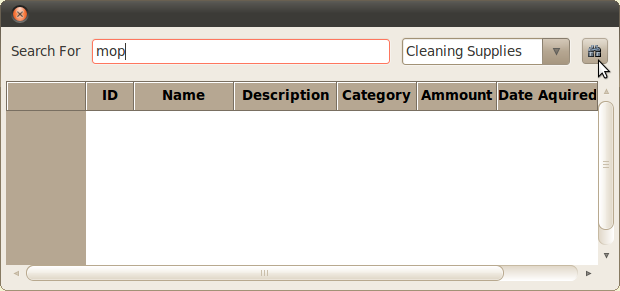
\includegraphics{ss3.png}}}
\caption{The user does a search to determine how many mops they have in the
office.}
\end{figure}

\begin{figure}[h!]
\center{\resizebox{280pt}{!}{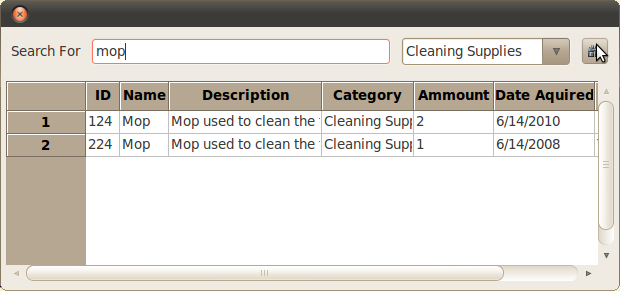
\includegraphics{ss4.png}}}
\caption{The search returns two entries for mop.}
\end{figure}

\begin{figure}[h!]
\center{\resizebox{280pt}{!}{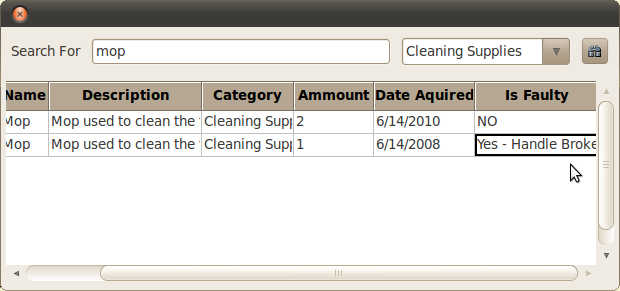
\includegraphics{ss6.png}}}
\caption{We see that the clinic was two good mops and on old broken one.}
\end{figure}

%\chapter*{}

The database search is carried out by converting the users search input
into a SQL query.  By using categories we can reduce the number of results
returned to the user.  This makes reading the results easier for the user.
The search is done case-insensitive, and the key word is searched against
the item name, item description, item ID, and the faulty description.

\chapter*{B}


\end{document}

